\documentclass{article}
\usepackage[T1]{fontenc}
\usepackage{lmodern}
\usepackage{graphicx}
\usepackage{amsmath,amssymb}
\usepackage[a4paper,margin=2cm]{geometry}
\usepackage[absolute,overlay]{textpos}
\setlength{\TPHorizModule}{1mm}
\setlength{\TPVertModule}{1mm}
\usepackage[indonesian]{babel}
\usepackage{hyperref}
\setlength{\emergencystretch}{2em}
% unit: Halaman 49

\begin{document}

% === Halaman 49 (llm) ===

Pergeseran warna sebesar 1 dari 256 warna tidak dapat dilihat oleh manusia

\vspace{20mm}

Sumber: TA Yulie Anneria Sinaga 13504085

% deskripsi: Gambar contoh steganografi yang menunjukkan foto paprika berwarna-warni dengan teks tersembunyi 'PESAN RAHASIA' dan deretan angka biner di sisi kanan.
% bbox normalisasi: [0.3300, 0.3200, 0.6670, 0.8870]
\begin{textblock*}{70.77mm}(69.30mm,95.04mm)
\noindent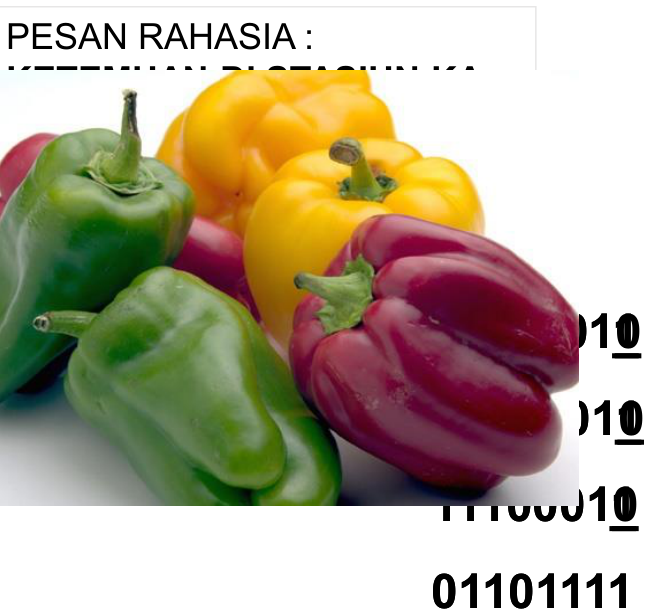
\includegraphics[width=70.77mm,height=168.40mm]{../../images/llm/page_049_img_01.png}%
\end{textblock*}

\end{document}
